\section{Ordinateur Dell de type tour T1700/3620}

L'ordinateur que nous avons représenté dans ce TP est un ordinateur de type tour Dell T1700/3620. 

% Il contient :
% \begin{itemize}
%     \item La carte mère
%     \item Le processeur
%     \item La mémoire vive (RAM)
%     \item Le disque dur 
%     \item L'alimentation
%     \item La carte graphique
%     \item Le lecteur / graveur CD/DVD
% \end{itemize}

\subsection{La carte mère}

La carte mère utilisée dans cet ordinateur ( figure \ref{fig:carte-mere-dell} ) a été fabriqué en Chine et elle est composée de :
\begin{itemize}
    \item 54,18 g de condensateur, type électrolyte 
    \item 91,5 g de condensateur, pour montage en surface
    \item 81,2 g de connecteur électrique, bus d'interconnexion de composants périphériques
    \item 182 g de connecteur électrique, bus de type périphérique
    \item 17 g d'inducteur, puce multicouche de faible valeur
    \item 50 g de circuit intégré, type logique
    \item 6,71 $\times 10^4 mm^2$ de montage, technologie de montage en surface, soudure sans Pb
    \item 6,71 $\times 10^4 mm^2$ de carte de câblage imprimée, pour montage en surface, surface sans Pb
    \item 64 $mm^2$ Plaquette, fabriquée, pour circuit intégré
\end{itemize}

\begin{figure}[h]
    \begin{subfigure}[t]{0.47\textwidth}
        \centering
        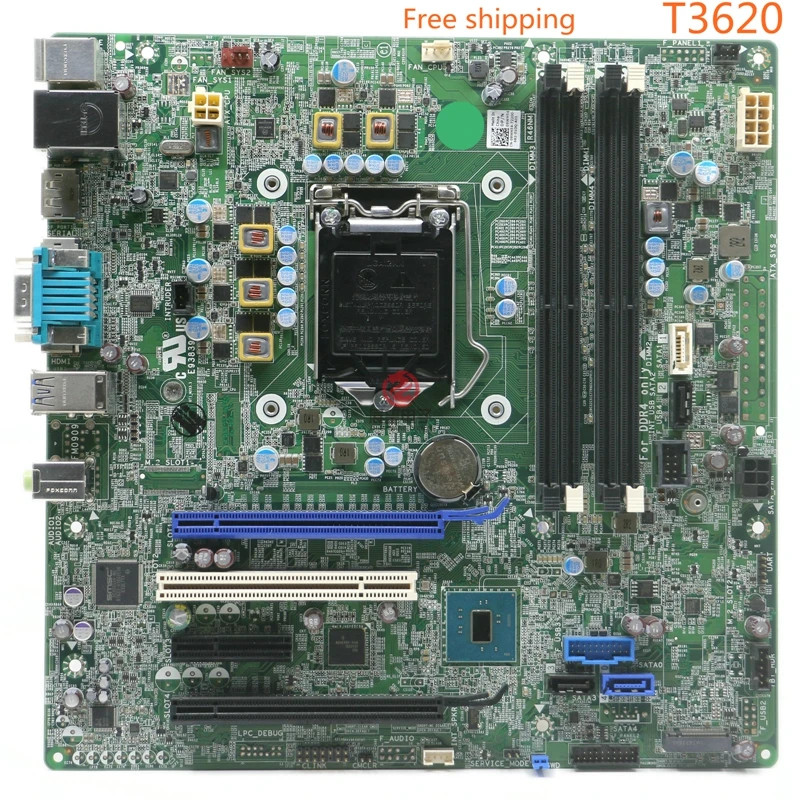
\includegraphics[width=\textwidth]{TP_2-Images_ordinateurs/dell_precision_tower_3620/precision_tower_3620-motherboard-aliexpress.jpg}
        \caption{Carte mère de l'ordinateur Dell T1700/3620}
        \label{fig:carte-mere-dell}
    \end{subfigure}
    \begin{subfigure}[t]{0.47\textwidth}
        \centering
        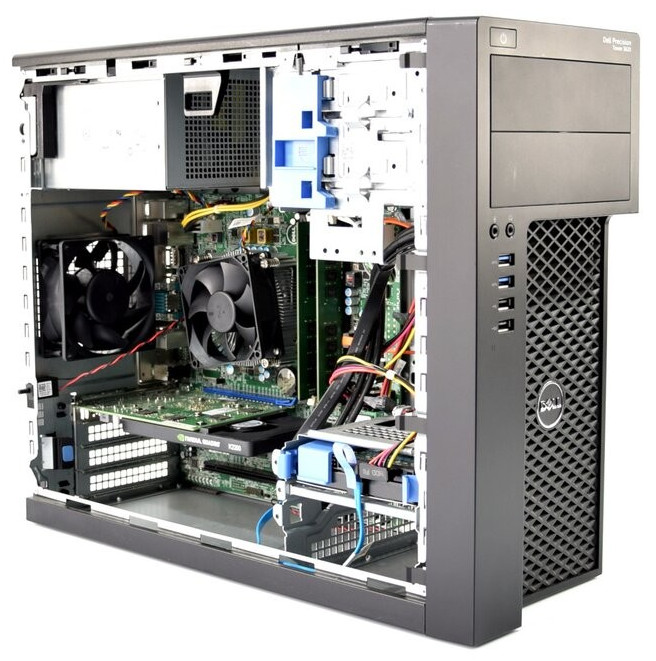
\includegraphics[width=\textwidth]{TP_2-Images_ordinateurs/dell_precision_tower_3620/precision_tower_3620-overview-mdm_komputery.jpg}
        \caption{Chassis de l'ordinateur Dell T1700/3620}
        \label{fig:chassis-dell}
    \end{subfigure}
    \caption{Carte mère et chassis de l'ordinateur Dell T1700/3620}
\end{figure}

\vspace{5pt}
Le problème de cette modélisation est la limitation aux composants principaux de la carte mère sans prendre en compte les autres composants qui la compose comme par exemple les dissipateurs thermiques et les composants de base comme le substrat FR4 et le cuivre dans les pistes.

De plus, le boitier de la carte mère n'est pas pris en compte ni son emballage.


\subsection{Le chassis de l'ordinateur}

\begin{itemize}
    \item 0,15 kg de copolymère acrylonitrile-butadiène-styrène
    \item 1,8 m de câble, connecteur pour ordinateur, sans fiches
    \item 3,0 m de câble, câble réseau, catégorie 5, sans fiches
    \item 0,05 kg de câble, câble plat, 20 broches, avec fiches
    \item 1 fiche, entrée et sortie, pour câble d'ordinateur
    \item 1 fiche, entrée et sortie, pour câble réseau
    \item 0,53 $m^2$ de peinture en poudre, acier
    \item 5 kg de laminage de tôles, acier
    \item 5 kg de acier, faiblement allié, laminé à chaud
    \item 0,15 kg de moulage par étirage-soufflage
    \item 1 ventilateur de 120 mm
    \item 1 ventilateur pour la tour
\end{itemize}

\vspace{5pt}

La modélisation du chassis ( figure \ref{fig:chassis-dell} ) est très simpliste car elle ne prend pas en compte les autres composants de la tour comme les vis, les entretoises, les plastiques de protection, le carton d'emballage et la colle. De plus, il n'y a pas de prise en compte des autres composants de la tour comme le lecteur/graveur CD/DVD et l'alimentation et 3 mètres de câble de réseau est beaucoup trop pour un ordinateur de bureau.

Neanmoins, la modélisation a aussi des points positifs comme la distinction de câble, les matériaux qui sont bien représenté et l'utilisation cohérente des unités.

\subsection*{Assemblage de l'ordinateur}

Dans \citep{hischier2007electronic}, il est décrit le processus de fabrication de l'ordinateur ainsi que les déchets provoqués par la fabrication de l'ordinateur.

Le processus d'assemblage de l'ordinateur consomme en moyenne 0,245 Kwh et 1,6 $m^3$ d'eau pour un ordinateur de type tour. 

\subsection{Comparaison du bilan carbone}

Après avoir modélisé l'ordinateur, pris en compte l'emballage et le transport depuis Chine jusqu'à en France, nous avons pu calculer le bilan carbone de l'ordinateur Dell T1700/3620 et nous avons obtenu un bilan carbone de 290,36 kgCO2 eq.

Dans l'étude fourni par DELL dans le document \citep{dell2018carbon}, il est indiqué que le bilan carbone de l'ordinateur est de 340,26 kgCO2 eq.

Cette différence peut être expliquée par le fait que nous n'avons pas pris en compte les autres composants de l'ordinateur comme le lecteur/graveur CD/DVD, l'alimentation et les autres composants de la carte mère. De plus, nous n'avons pas pris en compte les autres composants de la tour comme les vis, les entretoises, les plastiques de protection, le carton d'emballage et la colle. Mais aussi sur le fait que le transport des ordinateurs ne se fasse pas vers la même destination.